% version 1.00, date 28/01/16, auteur Michel Cressant
\section*{Informations générales}

\begin{table}[H]
\centering
	\begin{tabularx}{16.8cm}{|X|X|}
	\hline
	\rowcolor{gray!40} Numéro du risque & Type du risque \\
	\hline
	002 & Mauvaise ambiance dans l'équipe / problème de cohésion \\
	\hline
	\end{tabularx}
\end{table}

\begin{table}[H]
\centering
	\begin{tabularx}{16.8cm}{|X|X|X|}
	\hline
	\rowcolor{gray!40} Date & Visa du \RQ & Visa du \CP \\
	\hline
	 28/01/16 & pgpic & pgpic \\
	\hline
	\end{tabularx}
\end{table}

\begin{table}[H]
\centering
	\begin{tabularx}{16.8cm}{|X|X|X|X|}
	\hline
	\rowcolor{gray!40} Pilote & Activité WBS & Compte WBS & Phase d'apparition \\
	\hline
	 \Michel & Suivre les Risques et Opportunités & 1.2.3.2 & À partir du début du projet\\
	\hline
	\end{tabularx}
\end{table}

\section*{Description du risque}

\subsection*{Résumé}
	Le risque lié à la mauvaise ambiance dans le \PICCourt{} ou au problème de cohésion  peut entraîner une mauvaise façon de travailler et donc influencer la qualité du produit finale.
	
\subsection*{Analyse des causes}
	voir figure \ref{risque mauvaise ambiance dans l'équipe et mauvaise cohesion}. 

\subsection*{Criticité}

\begin{table}[H]
\centering
	\begin{tabularx}{16.8cm}{|>{\columncolor{gray!40}}X|X|}
	\hline
	Gravité & 3\\
	\hline
	Probabilité & 2\\
	\hline
	Criticité & A surveiller\\
	\hline
	\end{tabularx}
\end{table}
\newpage

\section*{Actions}
\subsection*{Actions préventives}

%\begin{table}[H]
\centering
	\begin{longtable}{|p{7cm}|p{7cm}|}
	\hline
	\rowcolor{gray!40} Numéro de cause & Actions préventives \\
	\hline
	 1 & \begin{itemize}
	 	\item Mettre en place des Team Building
	 	\item L'équipe établit des règles communes de fonctionnement des \PICCourt{}
	 	\item Le chef projet met en place des règles de communication de type DESC
	 \end{itemize} \\
	\hline
	2 & \begin{itemize}
		\item Entraide de l'équipe
		\item Partage du travail
	\end{itemize}	 \\
	\hline
	3 & \begin{itemize}
		\item Soutien moral
	\end{itemize} \\
	\hline
	
	\end{longtable}
%\end{table}

\flushleft
\subsection*{Plan de contournement}

\begin{enumerate}
	\item Le chef de projet identifie l'objet du conflit et interroge chaque membre concerné.
	\item Le chef de projet prend le rôle de médiateur et convoque les membres concernés à une réunion de négociation puis leur demande de mettre en oeuvre la méthode DESC.
\end{enumerate}

\section*{Décision de clôture}
Par le \CP{} et le pilote du risque.
\begin{table}[H]
\centering
	\begin{tabularx}{16.8cm}{|X|X|}
	\hline
	\rowcolor{gray!40} Date de clôture & Raison de la clôture \\
	\hline
	  & \\
	\hline
	\end{tabularx}
\end{table}

\section*{Historique des modifications}
\begin{table}[H]
\centering
	\begin{tabularx}{16.8cm}{|X|X|}
	\hline
	\rowcolor{gray!40} Date & Modification \\
	\hline
	  & \\
	\hline
	\end{tabularx}
\end{table}
\newpage

\begin{figure}
	\centering
	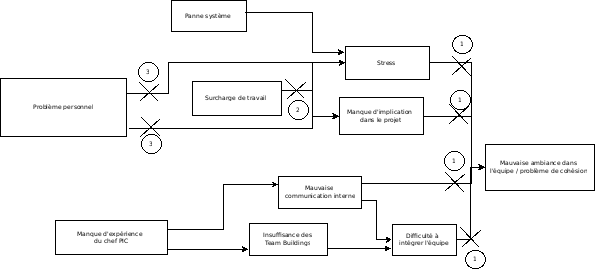
\includegraphics[scale=0.6]{images/AnalyseRisque_nPourquoi_FDR002}
	\caption{\label{risque mauvaise ambiance dans l'équipe et mauvaise cohesion}Risque mauvaise ambiance dans l'équipe et mauvaise cohésion - méthode des n pourquoi}
\end{figure}
